\section{Durchführung}

\subsection{Versuchsaufbau}
Ein Schaltplan des Versuchsaufbaus ist in Abbildung \ref{fig:schaltung} zu sehen.
\begin{figure}[H]
    \centering
    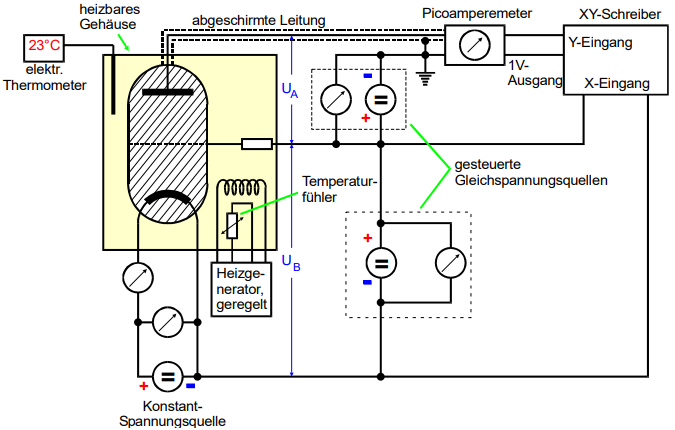
\includegraphics[height = 7.5cm]{bilder/schaltung.png}
    \caption{Schaltplan des Versuches \cite{man:v601}.}
    \label{fig:schaltung}
\end{figure}

\noindent
Das Glasrohr mitsamt der Elektroden, dem Glühdraht und dem Hg-Dampf befinden sich in einem heizbaren Gehäuse.
Die Innentemperatur $T$ kann mittels eines elektronischen Temperaturreglers eingestellt werden.
%wobei hier allerdings Schwankungen auftreten.
Die Temperatur selbst kann an einem elektronischen Thermometer abgelesen werden.
Der Glühdraht ist an eine Konstantspannungsquelle angeschlossen.
Die Beschleunigungselektrode ist an eine Gleichspannungsquelle angeschlossen, deren Variationsbereich zwischen 0 und $\qty{60}{\volt}$ liegt.
Die Spannungsquelle der Auffängerelektrode hat einen Bereich von 0 bis $\qty{11}{\volt}$.
Mit Hilfe eine Picoamperemeters kann der Auffängerstrom $I_\text{A}$ gemessen werden.
Der Strom $I_\text{A}$ kann mit Hilfe eines xy-Schreibers je nach Messreihe in Abhängigkeit von $U_\text{A}$ bzw. $U_\text{B}$ aufgezeichnet werden.
Die Spannung liegt dabei am x-Eingang und der Strom am y-Eingang.
Die Spannung, die der y-Eingang benötigt, kommt dabei aus dem Picoamperemeter.


\subsection{Energieverteilung der Elektronen}
\textbf{WERTE PRÜFEN/ EINGEBEN!!!!!}
Zum Messen der integrablen Energieverteilung der Elektronen wird eine konstante Beschleunigungsspannung $U_\text{B} = \qty[]{10}{\volt}$ eingestellt.
Am x-Ausgang des xy-Schreibers wird $U_\text{A}$ angelegt.